%%%%%%%%%%%%%%%%%%%%%%%%%%%%%%%%%%%%%%%%%
% University/School Laboratory Report
% LaTeX Template
% Version 4.0 (March 21, 2022)
%
% This template originates from:
% https://www.LaTeXTemplates.com
%
%%%%%%%%%%%%%%%%%%%%%%%%%%%%%%%%%%%%%%%%%

%----------------------------------------------------------------------------------------
%	PACKAGES AND DOCUMENT CONFIGURATIONS
%----------------------------------------------------------------------------------------

\documentclass[
	a4paper, % Paper size, specify a4paper (A4) or letterpaper (US letter)
	10pt, % Default font size, specify 10pt, 11pt or 12pt
]{CSUniSchoolLabReport}

\addbibresource{sample.bib} % Bibliography file (located in the same folder as the template)

%----------------------------------------------------------------------------------------
%	REPORT INFORMATION
%----------------------------------------------------------------------------------------

\title{Report 4: Partial Differnetial Equations (PDEs)} % Report title

\author{Simon \textsc{Blaue}} % Author name(s), add additional authors like: '\& James \textsc{Smith}'

\date{\today} % Date of the report

%----------------------------------------------------------------------------------------

\begin{document}

\maketitle % Insert the title, author and date using the information specified above


\begin{tabular}{l r}
	Universität Göttingen \\ % Date the experiment was performed
	Faculty of Physics \\
	Instructor: Prof. Dr. S. Schumann \\
	Tutors: Dr. E. Bothmann, M. Knobbe \\ % Partner names
\end{tabular}


% If you need to include an abstract, uncomment the lines below
%\begin{abstract}
%	Abstract text
%\end{abstract}

\vspace*{50px}
%----------------------------------------------------------------------------------------
%	CONTENT
%----------------------------------------------------------------------------------------

\section{Laplace Equation}

\subsection{Iterator methods}

\begin{figure}[H]
	\centering
	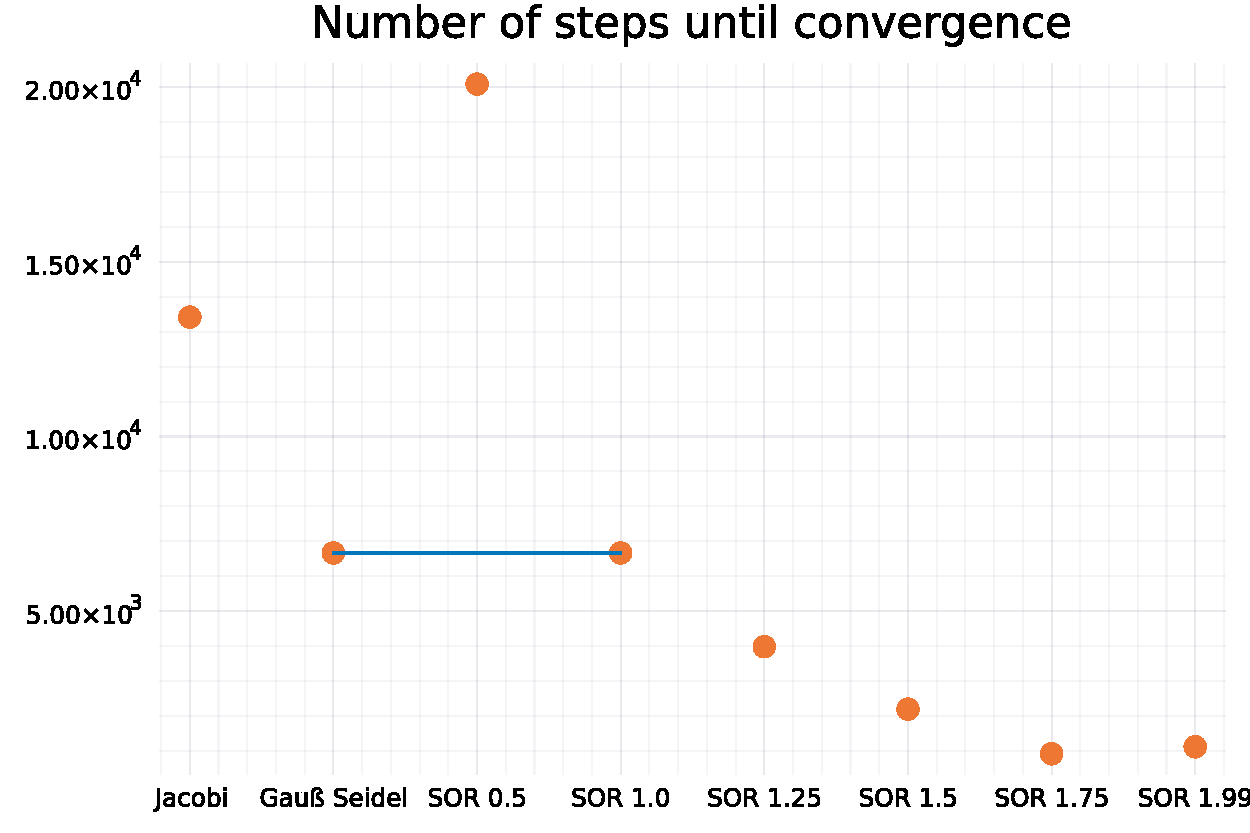
\includegraphics[width=\textwidth]{../saves/number_of_convergence_steps.pdf}
	\caption{Number of steps until convergence concerning the Laplace error $\max\epsilon<1\times 10^{-3}$.}
\end{figure}


\begin{figure}[H]
	\centering
	\begin{subfigure}[b]{0.49\textwidth}
			\centering
			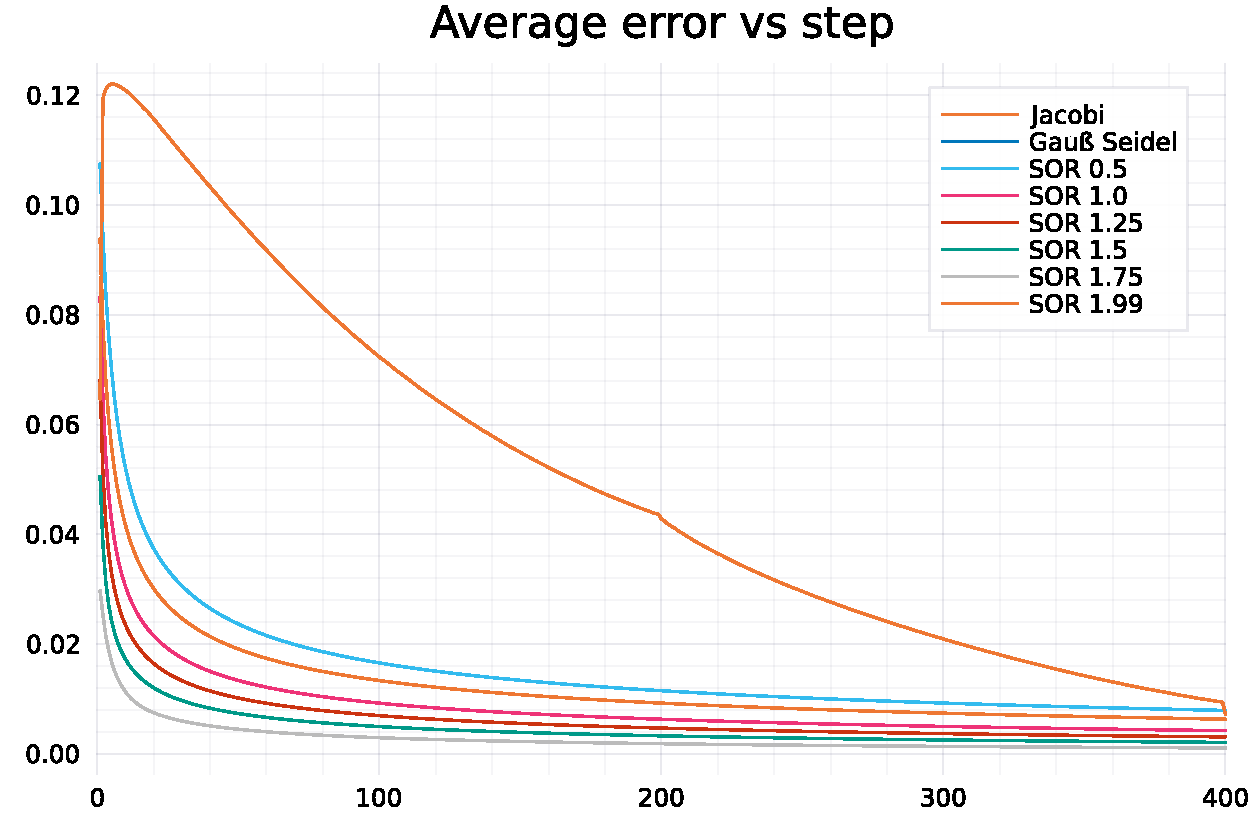
\includegraphics[width=\textwidth]{../saves/av_errors_comp.pdf}

			\label{fig:av_errors}
	\end{subfigure}
	\hfill
	\begin{subfigure}[b]{0.49\textwidth}
			\centering
			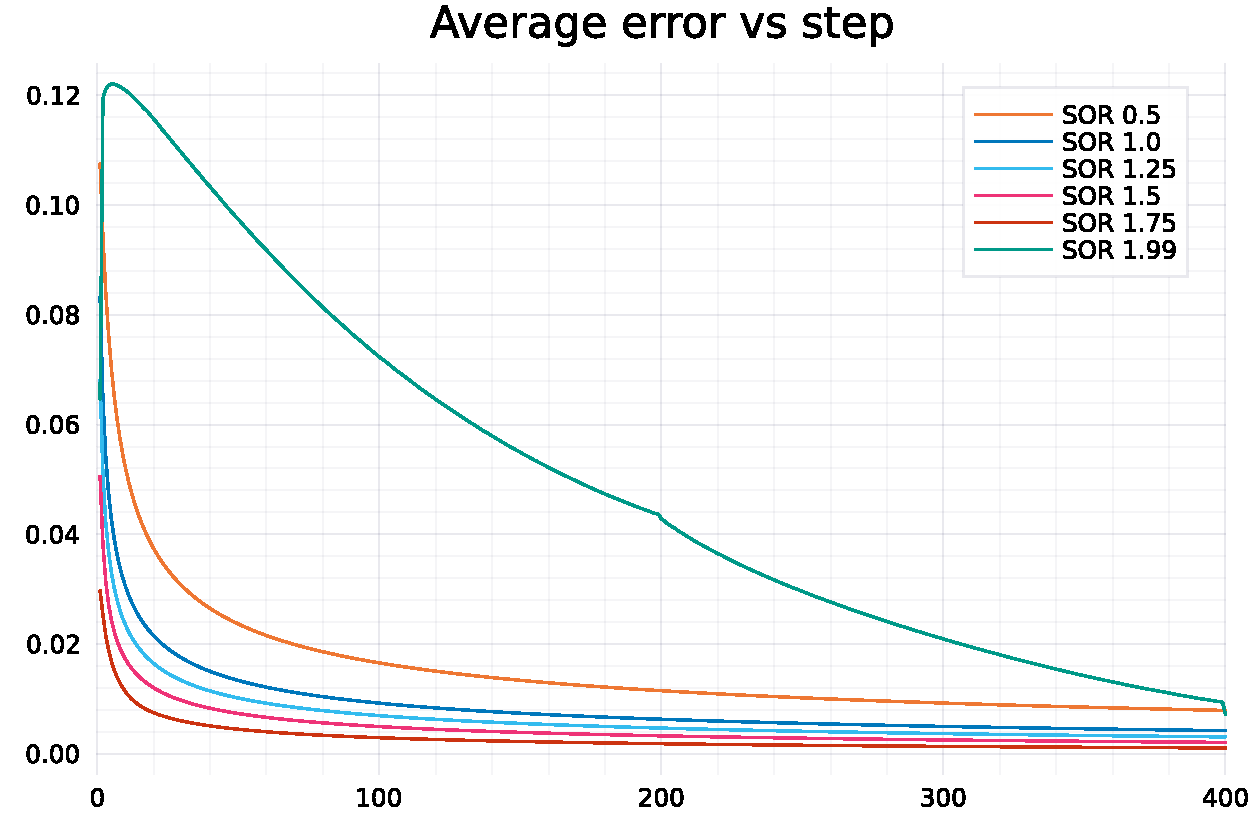
\includegraphics[width=\textwidth]{../saves/av_errors_SOR_comp.pdf}

			\label{fig:av_errors_SOR}
	\end{subfigure}
	\hfill
	\begin{subfigure}[b]{0.49\textwidth}
			\centering
			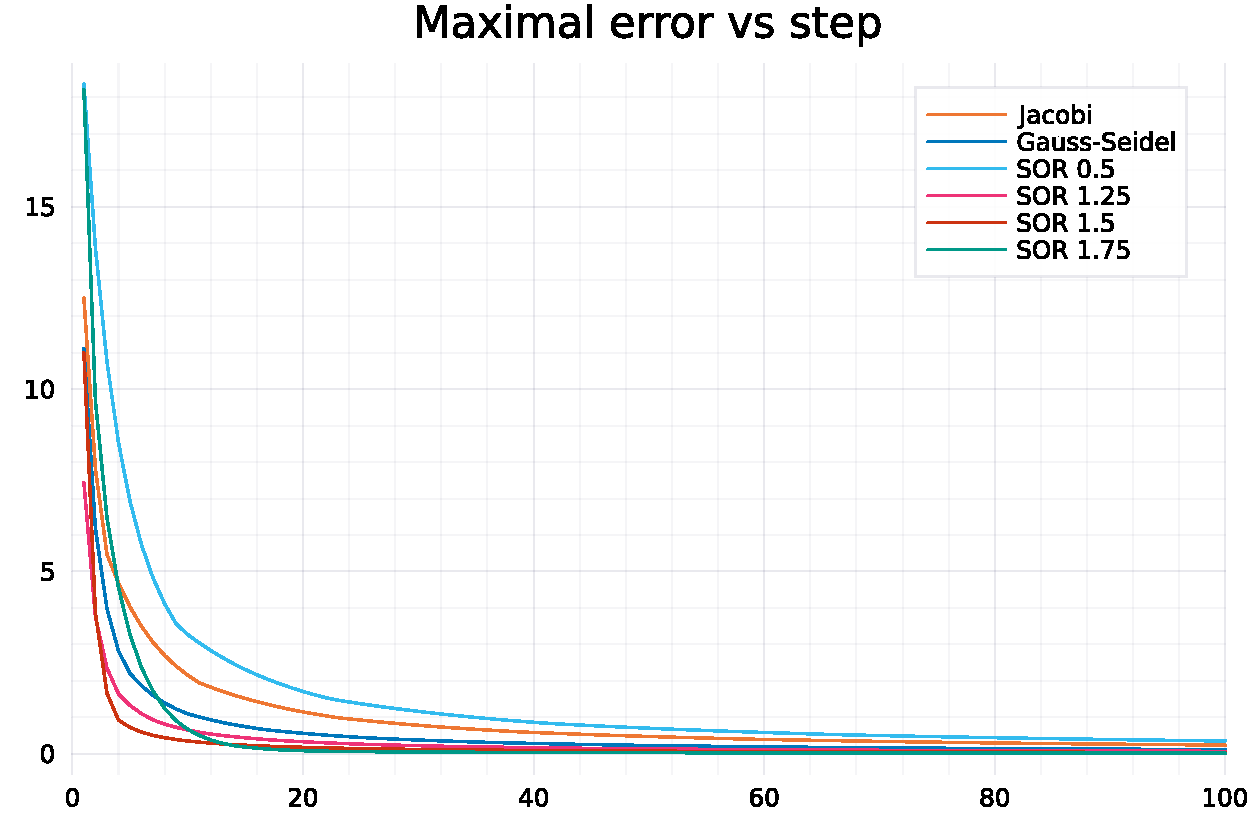
\includegraphics[width=\textwidth]{../saves/max_errors_comp.pdf}

			\label{fig:max_errors}
	\end{subfigure}
	\hfill
	\begin{subfigure}[b]{0.49\textwidth}
		\centering
		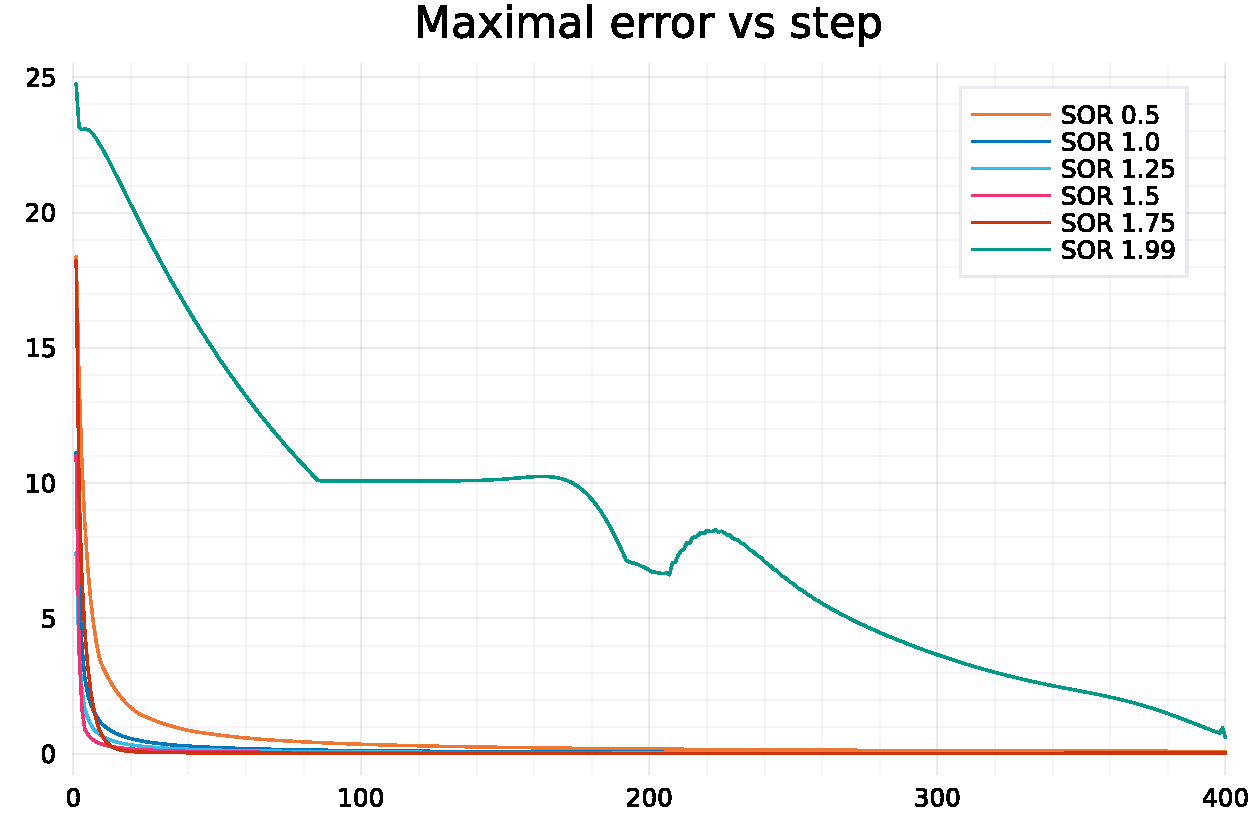
\includegraphics[width=\textwidth]{../saves/max_errors_SOR_comp.pdf}

		\label{fig:max_errors_SOR}
\end{subfigure}
		 \caption{Maximal and average error for different iteration methods.}
		 \label{fig:errors}
\end{figure}

\subsection{SOR for $\alpha=2.0$}

\begin{figure}[H]
	\centering
	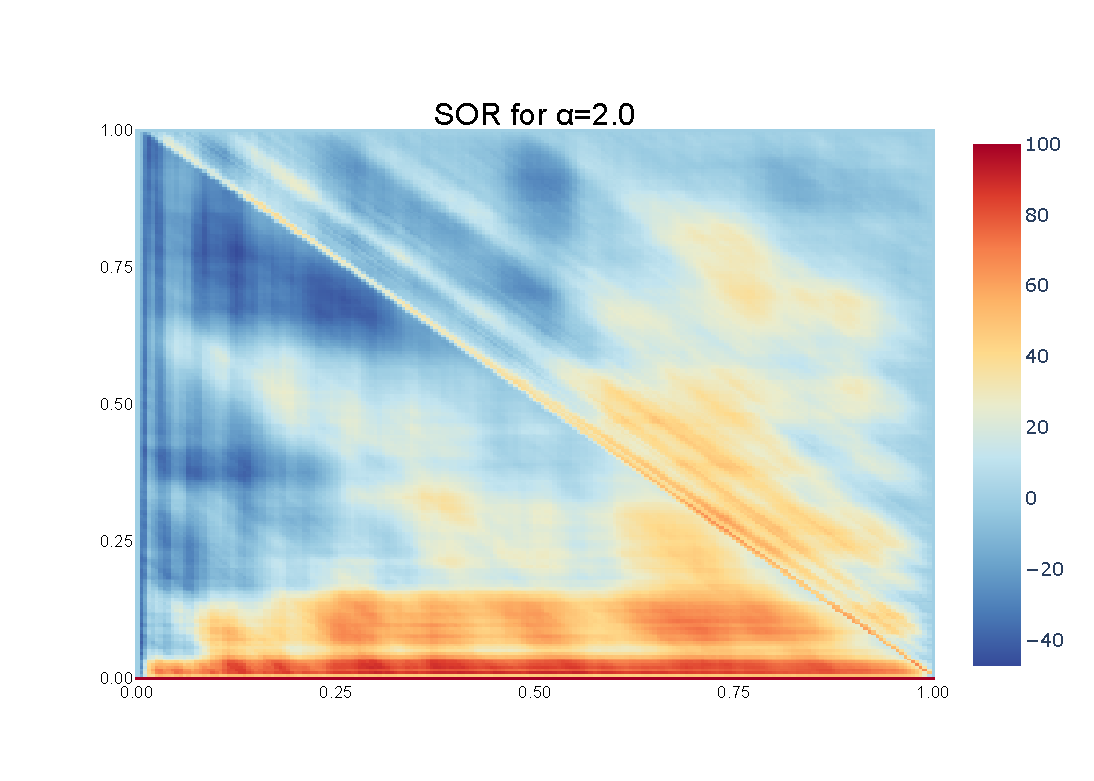
\includegraphics[width=\textwidth]{../saves/broken_SOR_heatmap.pdf}
	\caption{}
\end{figure}

\begin{figure}[H]
	\centering
	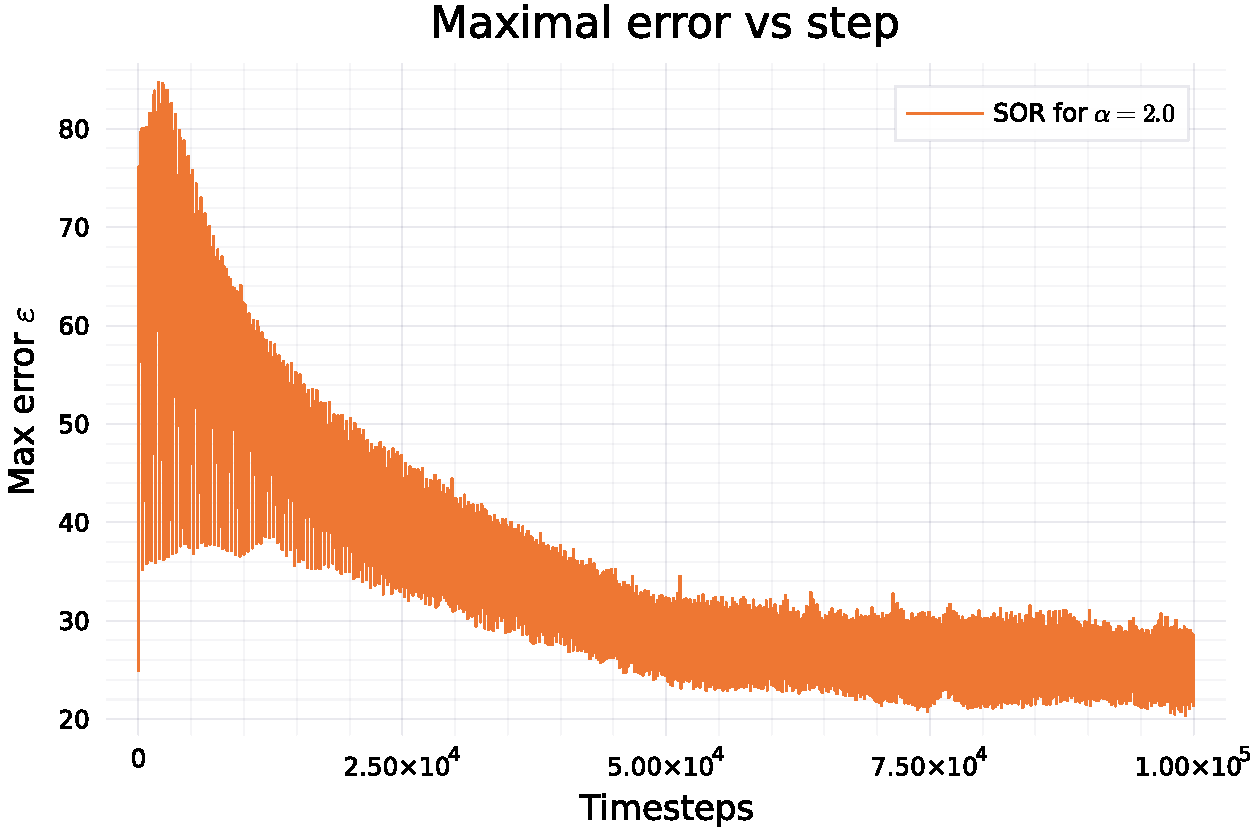
\includegraphics[width=\textwidth]{../saves/broken_SOR_error.pdf}
	\caption{}
\end{figure}

\subsection{Infinite sum solution}

\begin{figure}[H]
	\centering
	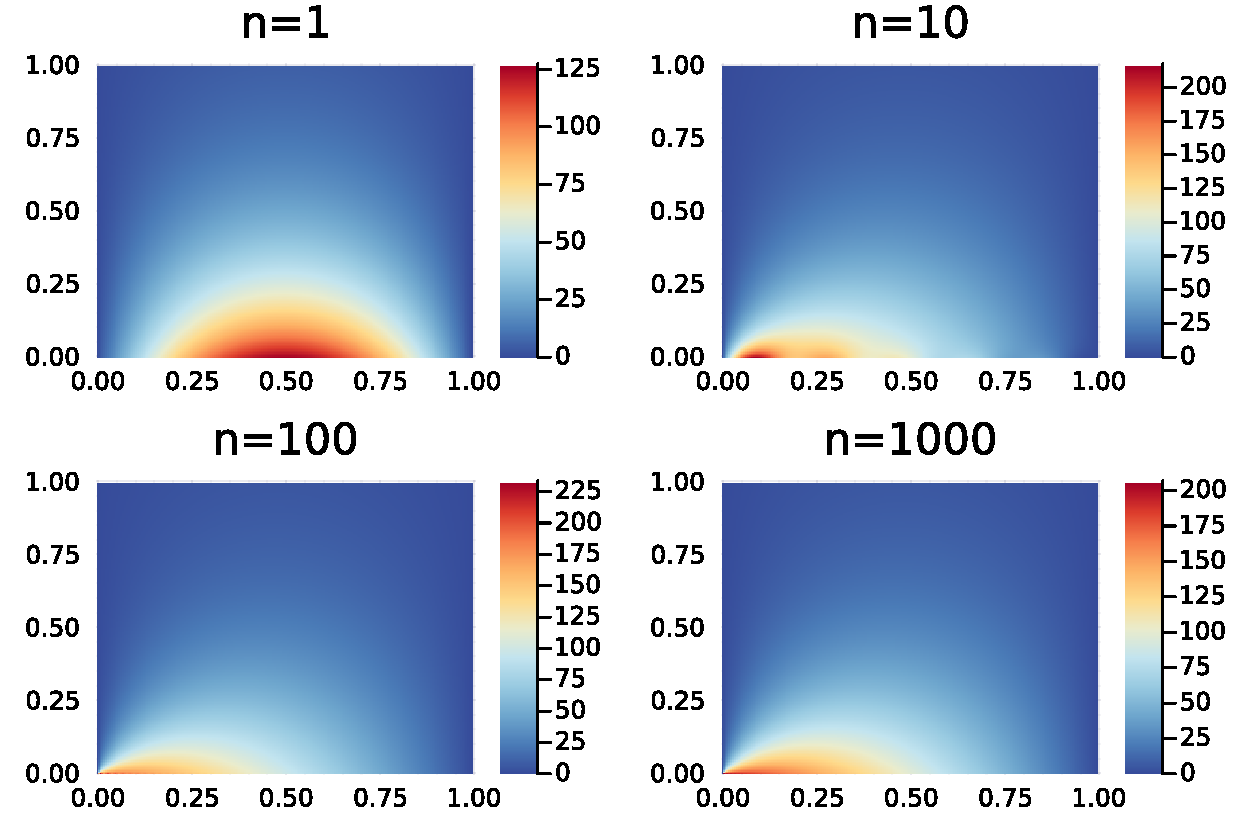
\includegraphics[width=\textwidth]{../saves/comp_lapplace_series_heatmap.pdf}
	\caption{Results for the "infinite" sum solution to the Laplace equation for different numbers of terms $n$.}
\end{figure}

\begin{figure}[H]
	\centering
	\begin{subfigure}[b]{\textwidth}
		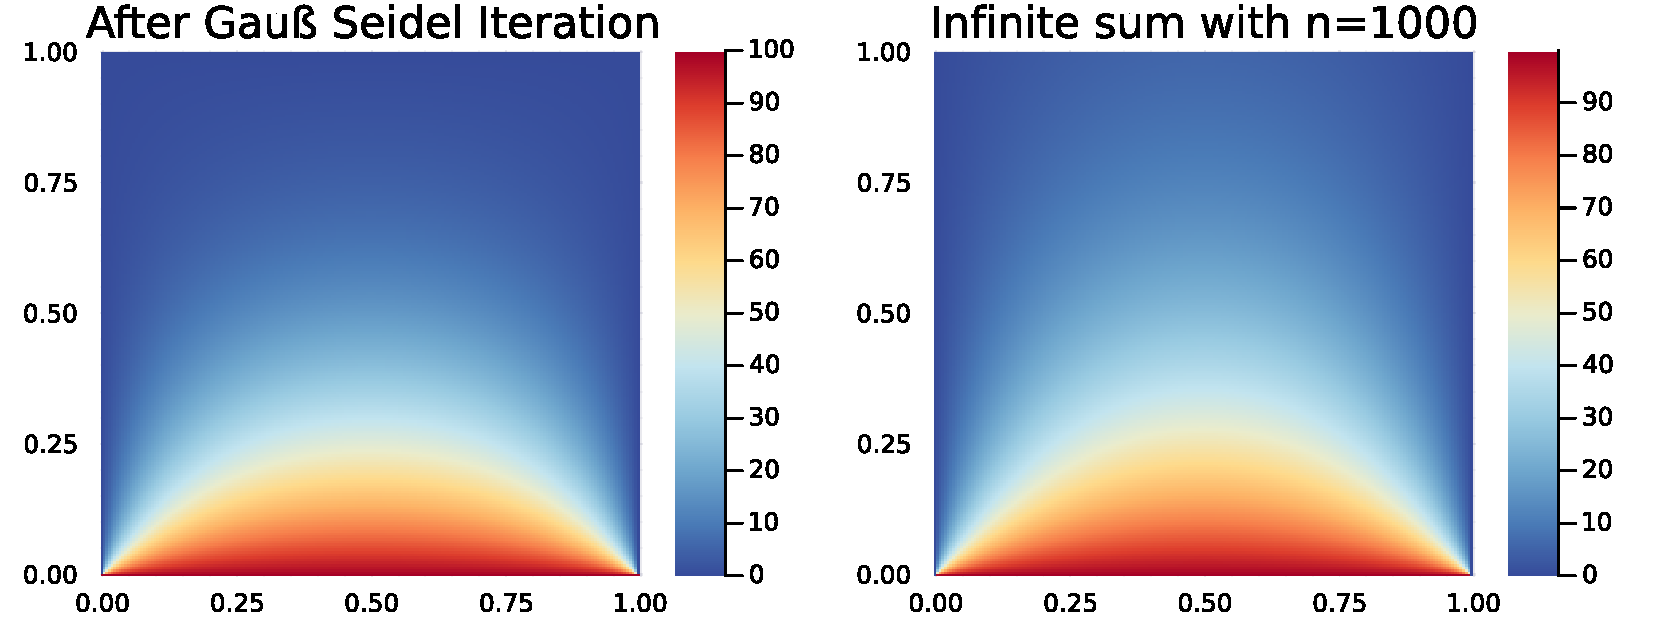
\includegraphics[width=\textwidth]{../saves/comp_laplace_heatmap.pdf}
		\caption{Comparison of the infinite sum solution with 1000 terms and the Gauß Seidel iterator solution.}
	\end{subfigure}
	\hfill
	\centering
	\begin{subfigure}[b]{0.6\textwidth}
		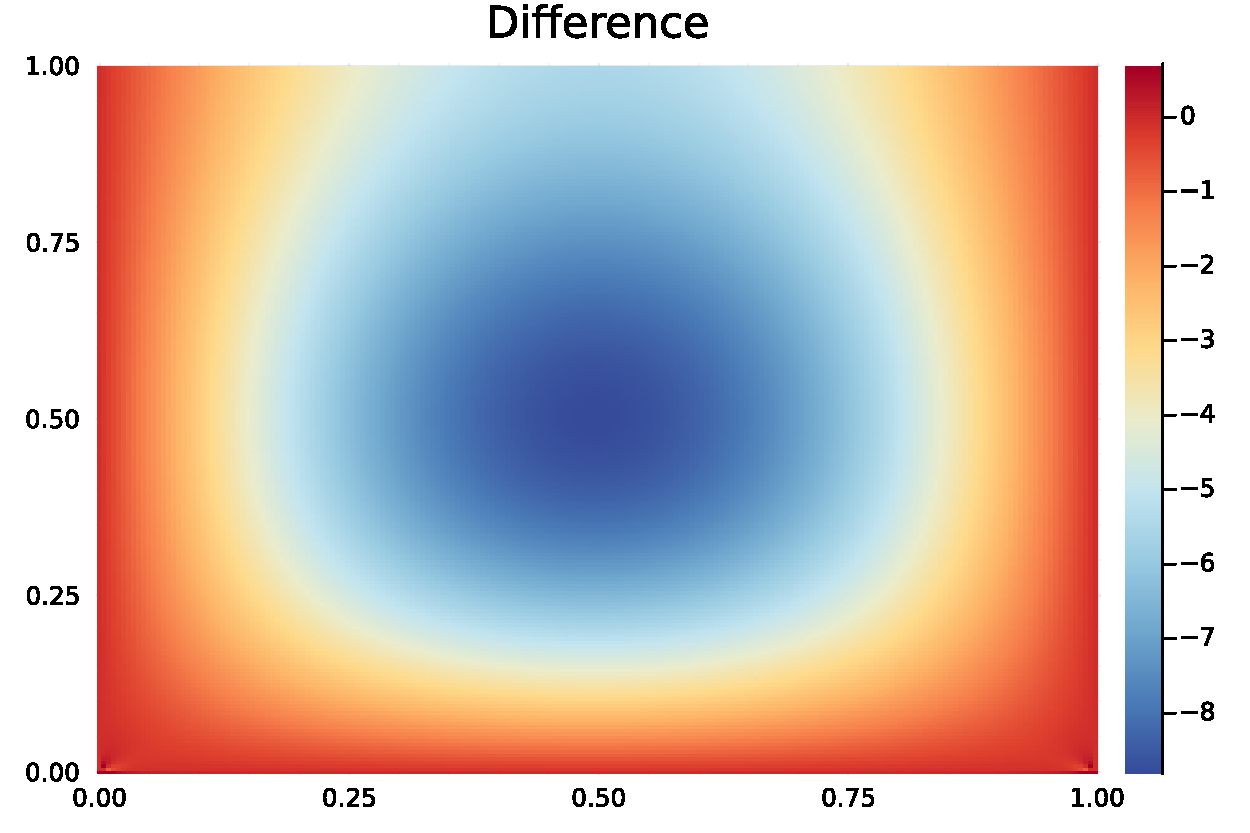
\includegraphics[width=\textwidth]{../saves/difference_laplace_heatmap.pdf}
		\caption{Difference between the infinite sum solution with 1000 terms and the Gauß Seidel iterator solution.}
	\end{subfigure}
\end{figure}


\section{Diffusion}

\subsection{Integration methods}

\begin{figure}[H]
	\centering
	\begin{subfigure}[b]{0.49\textwidth}
		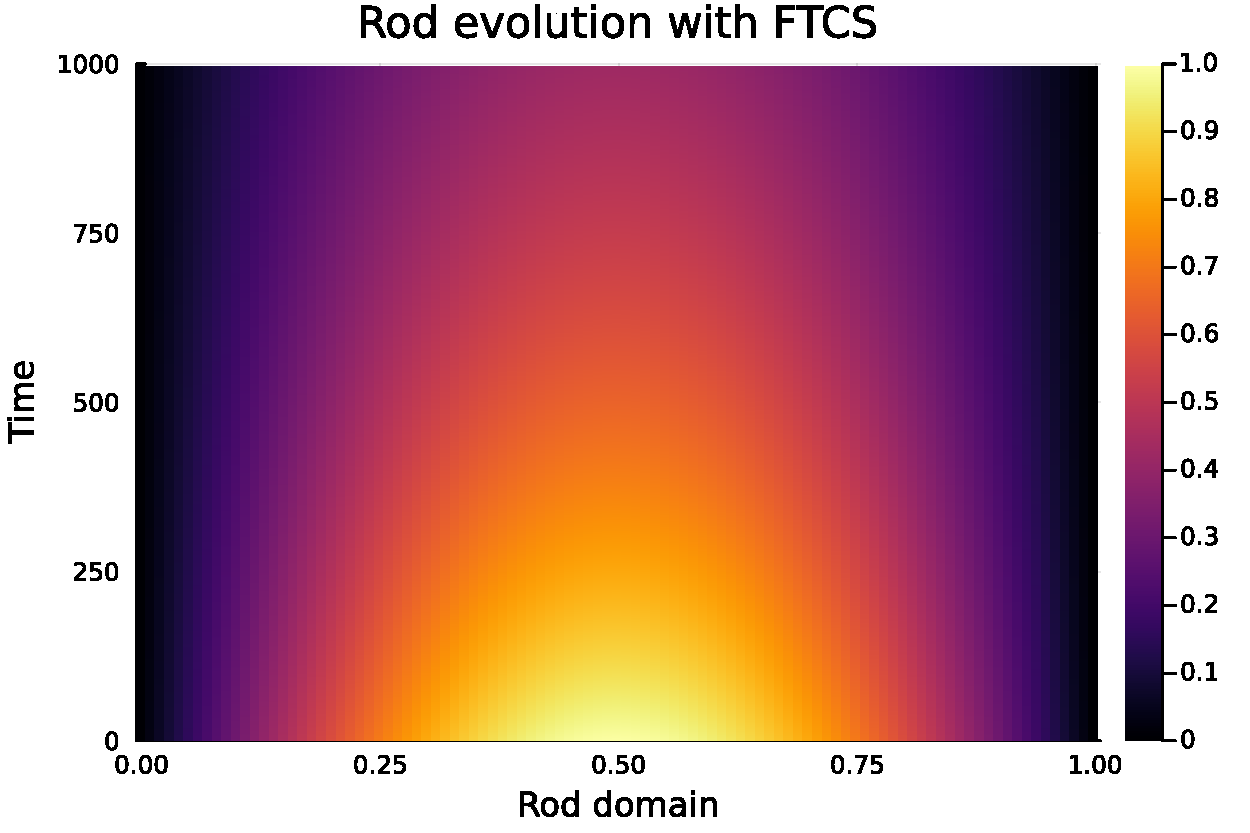
\includegraphics[width=\textwidth]{../saves_t2/rod_FTCS.pdf}
	\end{subfigure}
	\hfill
	\begin{subfigure}[b]{0.49\textwidth}
		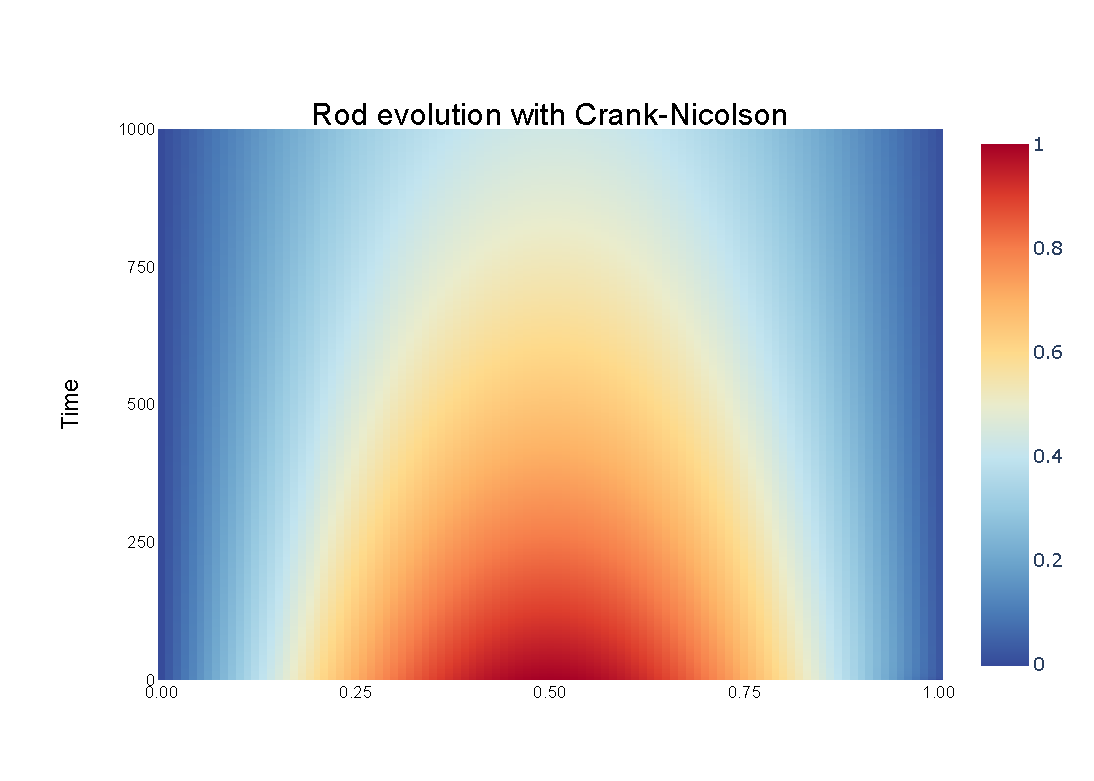
\includegraphics[width=\textwidth]{../saves_t2/rod_crank-nic.pdf}
	\end{subfigure}
	\hfill
	\begin{subfigure}[b]{0.49\textwidth}
		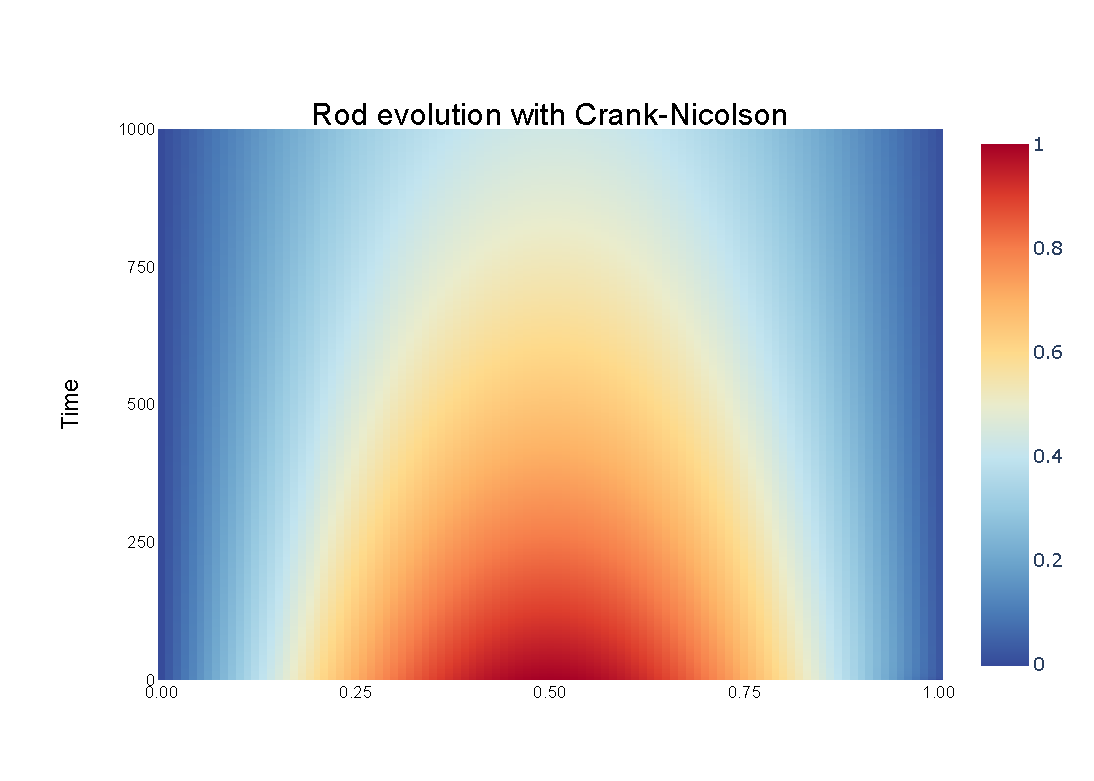
\includegraphics[width=\textwidth]{../saves_t2/rod_crank-nic.pdf}
	\end{subfigure}
	\hfill
	\begin{subfigure}[b]{0.49\textwidth}
		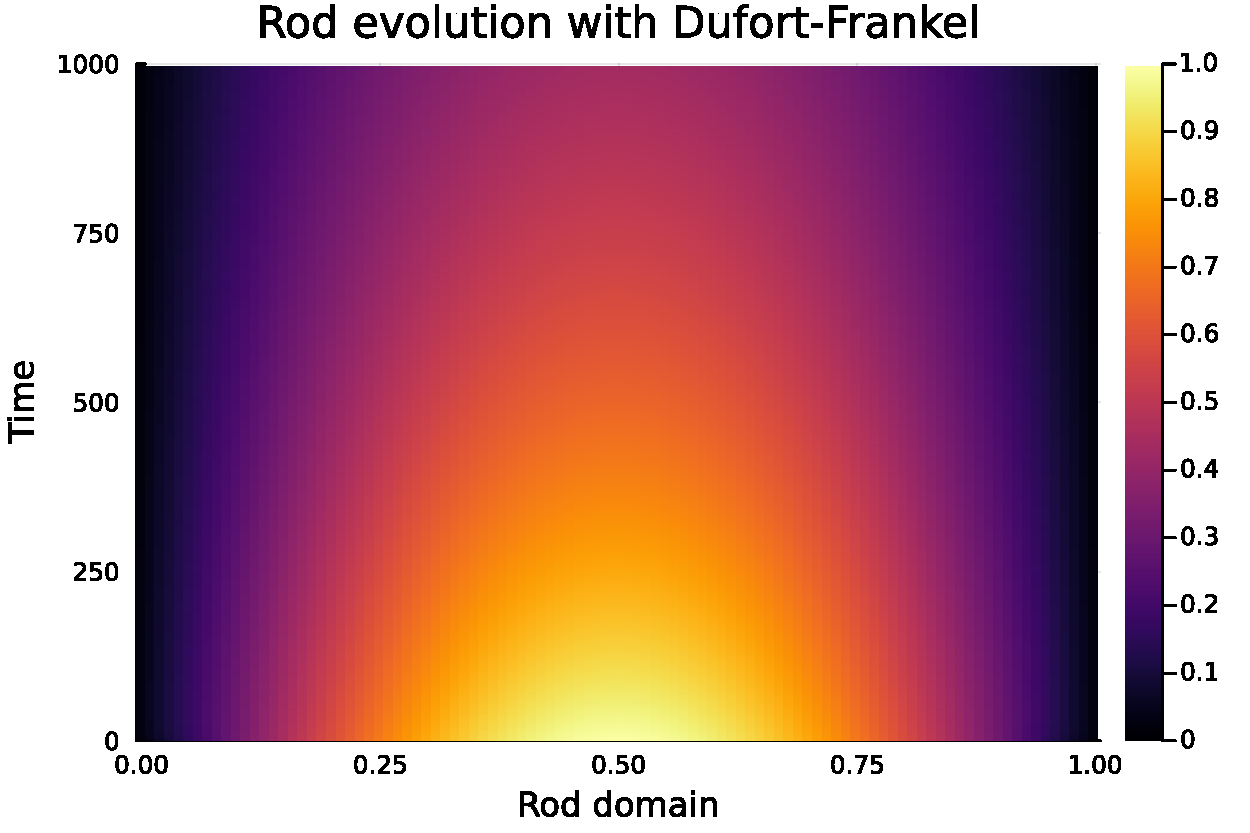
\includegraphics[width=\textwidth]{../saves_t2/rod_dufort_frankel.pdf}
	\end{subfigure}
	\hfill
	\caption{Temporal evolution of the rod's temperature along the y-axis. The evolution seems to be the same for all four integration methods.}
\end{figure}

\subsection{Error comparison}

\begin{figure}[H]
	\centering
	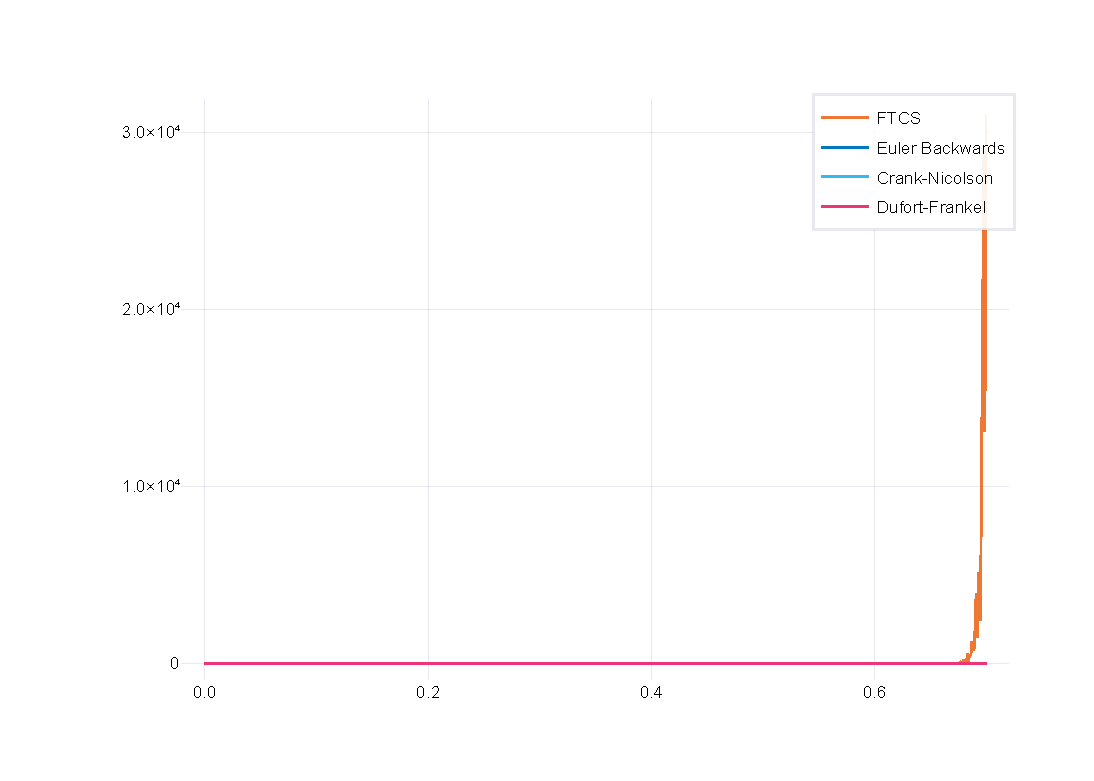
\includegraphics[width=\textwidth]{../saves_t2/error_comp.pdf}
	\caption{}
\end{figure}


\begin{figure}[H]
	\centering
	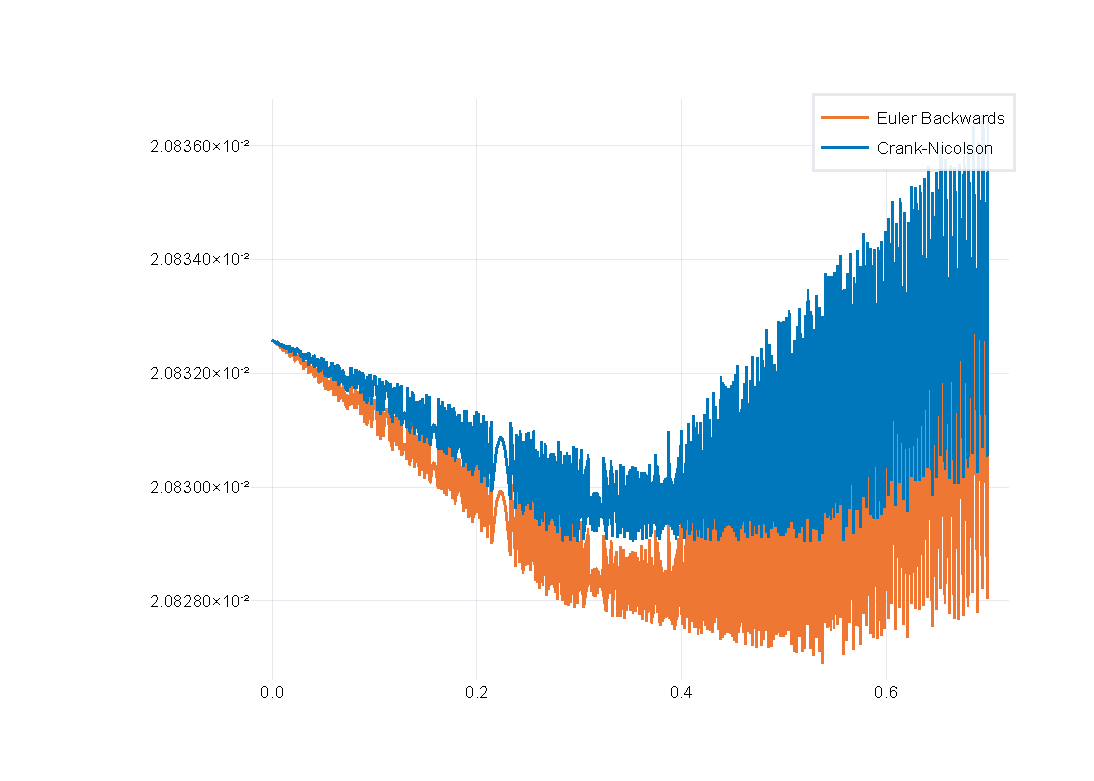
\includegraphics[width=\textwidth]{../saves_t2/error_comp_be_cn.pdf}
	\caption{}
\end{figure}


TODO: Dufort Franke not so nice
\begin{figure}[H]
	\centering
	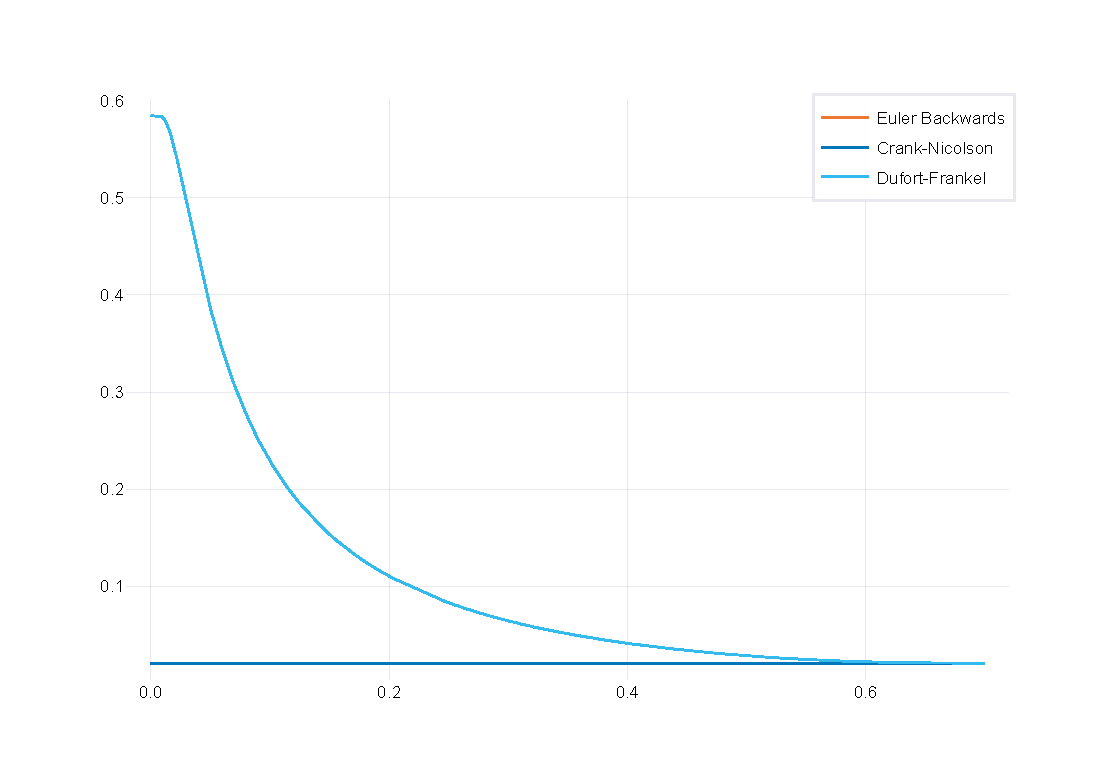
\includegraphics[width=\textwidth]{../saves_t2/error_comp_be_cn_df.pdf}
	\caption{}
\end{figure}


\section{Solitons}


%----------------------------------------------------------------------------------------
%	DISCUSSION
%----------------------------------------------------------------------------------------

% \section{Discussion}



%----------------------------------------------------------------------------------------
%	BIBLIOGRAPHY
%----------------------------------------------------------------------------------------

% \printbibliography % Output the bibliography

%----------------------------------------------------------------------------------------

\end{document}